% !TeX document-id = {b5392a94-51a3-49d1-9ba5-698bc09f9d35}
% !TeX encoding = UTF-8
% !TeX spellcheck = en_US
% !TeX TS-program = pdflatex
% !TeX TXS-program:bibliography = biber -l zh__pinyin --output-safechars %

\documentclass[a4paper
	,10pt
%	,twoside
]{article}

% to be `\input` in subfolders,
% ... therefore the path should be relative to subfolders.

\usepackage{iftex}
\ifPDFTeX
\else
	\usepackage[UTF8
		,heading=false
		,scheme=plain % English Document
	]{ctex}
\fi
%\ctexset{autoindent=true}
\usepackage{indentfirst}

\input{../.modules/basics/macros.tex}
\input{../.modules/preamble_base.tex}
\input{../.modules/preamble_beamer.tex}
\input{../.modules/basics/biblatex.tex}


%Misc
	\usepackage{lilyglyphs}
	\newcommand{\indicator}{$\text{\clefG}$}
	\newcommand{\indicatorInline}{$\text{\clefGInline}$}

\newcommand{\legacyReference}{{
%	\clearpage\par
%	\quad\clearpage
	\def{\midquote}{\textbf{PAST WORK, AS TEMPLATE}}
	\newparagraph
}}

% Settings
\counterwithout{equation}{section}
\mathtoolsset{showonlyrefs=false}
%\DeclareTextFontCommand{\textbf}{\sffamily}

% Spacing
\geometry{footnotesep=2\baselineskip} % pre footnote split
\setlength{\parskip}{.5\baselineskip}
\renewcommand{\baselinestretch}{1.15}


%% List
%	\setlist*{
%		listparindent=\parindent
%		,labelindent=\parindent
%		,parsep=\parskip
%		,itemsep=1.2\parskip
%	}


\addtobeamertemplate{navigation symbols}{}{%
    \usebeamerfont{footline}%
%    \usebeamercolor[fg]{footline}%
    \hspace{1em}%
    \large\insertframenumber/\inserttotalframenumber
}

\makeatletter
\setbeamertemplate{headline}
{%
    \begin{beamercolorbox}[wd=\paperwidth,colsep=1.5pt]{upper separation line head}
    \end{beamercolorbox}
    \begin{beamercolorbox}[wd=\paperwidth,ht=2.5ex,dp=1.125ex,%
      leftskip=.3cm,rightskip=.3cm plus1fil]{title in head/foot}
      \usebeamerfont{title in head/foot}\insertshorttitle
    \end{beamercolorbox}
    \begin{beamercolorbox}[wd=\paperwidth,ht=2.5ex,dp=1.125ex,%
      leftskip=.3cm,rightskip=.3cm plus1fil]{section in head/foot}
      \usebeamerfont{section in head/foot}%
      \ifbeamer@tree@showhooks
        \setbox\beamer@tempbox=\hbox{\insertsectionhead}%
        \ifdim\wd\beamer@tempbox>1pt%
          \hskip2pt\raise1.9pt\hbox{\vrule width0.4pt height1.875ex\vrule width 5pt height0.4pt}%
          \hskip1pt%
        \fi%
      \else%  
        \hskip6pt%
      \fi%
      \insertsectionhead
    \end{beamercolorbox}
% Code for subsections removed here
}
\makeatother
\input{../.modules/basics/biblatex.tex}

\title{A First Look at Celestial Holography}
\addbibresource{celestial.bib}

%%% ID: sensitive, do NOT publish!
\InputIfFileExists{id.tex}{}{}

\makeatletter
\newcommand{\nobeginpar}{\@beginparpenalty=10000}
\makeatother

\begin{document}
\maketitle
\pagenumbering{arabic}
\thispagestyle{empty}

%\vspace*{-.5\baselineskip}

\setlength{\parskip}{.1\baselineskip}
\tableofcontents
\setlength{\parskip}{\parskipnorm}

\addtocounter{section}{-1}
\section{References}
	\begin{itemize}
	\item \textbf{Primary reference:} \fullcite{Strominger:2017zoo}. 
	\item \textbf{Secondary:} \fullcite{Ball:2019atb}. 
	
	See also \fullcite{deBoer:2003vf}. 
	\item \textbf{Also:} \fullcite{Pate:2019mfs}
	\end{itemize}
	
	\noindent
	Talks by the authors:
	\begin{itemize}[noitemsep]
	\item Andy Strominger: \url{https://www.youtube.com/watch?v=By9hFSvl9MA}
	\item Monica Pate: \url{https://www.youtube.com/watch?v=4M4iZ8Hnc4Q}
	\item Andy Strominger, recent progress: \url{https://www.youtube.com/watch?v=wNLNIL81T_s}
	
	\vspace{.5\baselineskip}
	
	\item[**] Not very relevant, but there is a very recent, very interesting, very physical talk by Susskind at IAS on de Sitter holography: \url{https://www.youtube.com/watch?v=4GKjr-y5MY0}
	\end{itemize}

\pagebreak

\section{Basics}
\subsection{\textsl{What} is the celestial sphere?}
	The celestial sphere, \textkai{天球}, is a basic concept in astronomy. According to \href{https://en.wikipedia.org/wiki/Celestial_sphere}{\textsl{Wikipedia}}, the celestial sphere is an abstract sphere that has an arbitrarily large radius and is concentric to the observer. All objects in the sky can be conceived as being projected upon the inner surface of the celestial sphere. 
	
	The idea of celestial sphere in celestial holography is almost precisely the same as that in usual astronomy. Suppose we, the observers, are at the origin of a \textbf{asymptotically flat} universe; the stars we see in the sky are null rays coming from somewhere closed to the past null infinity $\mscr{I}^-$, i.e.~what we see in the night sky is precisely the celestial sphere $CS^-$ closed to $\mscr{I}^-$. Similarly, there is another celestial sphere $CS^+$ located near $\mscr{I}^+$. 
	
	\begin{figure}[!h]
	\centering
	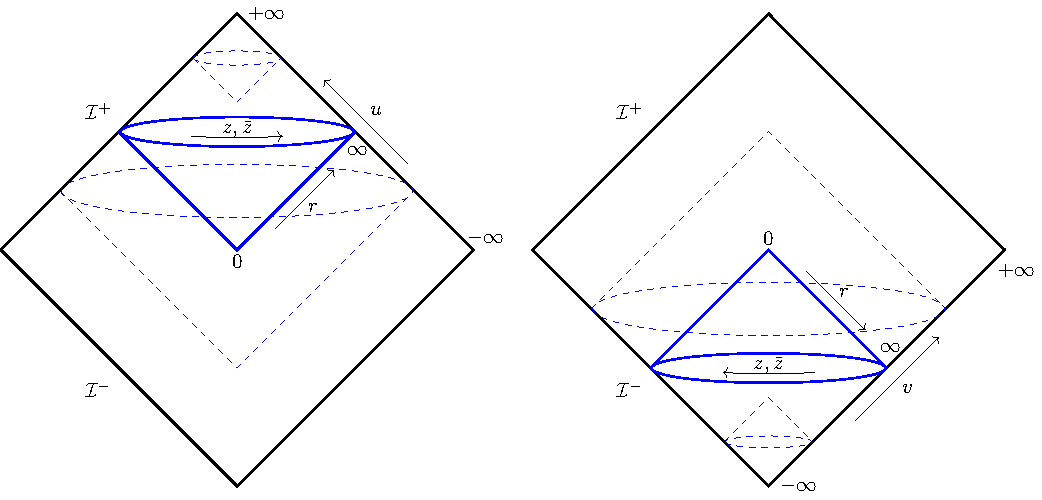
\includegraphics[width=.85\linewidth]{img/bond.pdf}
	\caption[Penrose diamond of Minkowski spacetime]{
		\textbf{Penrose \textsl{diamond}} of Minkowski spacetime, from \cite{Strominger:2017zoo}. Compared to the standard Penrose diagram, we can see the celestial sphere more clearly in this kind of diamond diagrams. Roughly speaking, we have $\mscr{I}^\pm = \mbb{R}^\pm \times CS^\pm$, where $\mbb{R}^\pm$ stands for the $u,v$ coordinates.
	}
	\end{figure}
	
	\textsl{We will primarily work in \textbf{4D}, where the celestial spheres} $CS^\pm \simeq S^2 \ni (z,\bar{z})$. 
	\begin{equation}
		\dd{s}^2
		= - \dd{u}^2 - 2\dd{u} \dd{r}
			+ r^2 \dd{\Omega}^2,
	\quad
		u = t - r,
	\end{equation}
	\vspace{-.8\baselineskip}
	\begin{equation}
		\dd{\Omega}^2
		= 2\gamma_{z\bar{z}} \dd{z} \dd{\bar{z}},
	\quad
		\gamma_{z\bar{z}}
		= \frac{2}{(1 + z\bar{z})^2}
	\label{eq:metric_null_plus}
	\end{equation}
	$u$: \textbf{retarded time}. 
	These coordinates work well near $\mscr{I}^+$ where $t,r\to\infty$ but $u = t - r$ stays finite. It's no good around $\mscr{I}^-$ where $u\to -\infty$; instead we need \textbf{advanced coordinates}:
	\begin{equation}
		\dd{s}^2
		= - \dd{v}^2
			\mathbin{\sidenote{+}} 2\dd{v} \dd{r}
			+ r^2 \dd{\Omega}^2,
	\quad
		v = t + r,
	\end{equation}
%	\meaning\sidenote
	
\pagebreak[4]
	Note that the $(z,\bar{z})$ in $CS^\pm$ are actually \textbf{not the same coordinates}, but are related to each other by the \textbf{antipodal map}:
	\begin{equation}
		z \mapsto -\frac{1}{\bar{z}},
	\quad
		\text{i.e.}\,\ %
		z_+ = - \frac{1}{\bar{z}_-},
	\ %
		z_- = - \frac{1}{\bar{z}_+},
	\end{equation}
	This is actually the more natural choice: a ``free'' light ray starting from $z_- = z$ ends at $z_+ = z$. This in fact binds $\mcal{I}^+$ with $\mcal{I}^-$. 
	
	Now consider a scattering process happening ``around $i^0$'', from $\mscr{I}^-$ to $\mscr{I}^+$; this is ``far away'' from the ``center'' where all the interactions take place, so the scattering process is almost trivial. 
	This gives the natural \textbf{antipodal matching condition} for fields around $i^0$:
	\begin{equation}
	\arraycolsep=.25em
	\begin{array}{ccccccccc}
		F(u,z,\bar{z})|_{\mscr{I}^+\to i^0}
		&=& F(u\to -\infty,z,\bar{z})
		&\equiv& F(z,\bar{z})
		&=& F(v\to +\infty,z,\bar{z})
		&=& F(v,z,\bar{z})|_{\mscr{I}^-\to i^0}
	\end{array}
	\end{equation}
	Note that this antipodal matching condition will prove crucial to our discussions later on. 
\subsection{\textsl{Why} do we want to study that?}
	\begin{enumerate}
	\item As an approach to \textbf{flat holography}. Another interesting observation: one can do some sort of a ``double holography'' by \textit{uplifting} $\mrm{AdS}_3/\mrm{CFT}_2$; this discussed in e.g.~\cite{deBoer:2003vf,Ball:2019atb}. 
	
	\begin{figure}[!h]
	\centering
	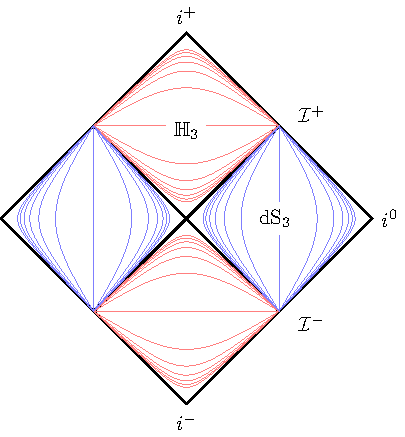
\includegraphics[width=.45\linewidth]{img/hyperbolicslicing.pdf}
	\caption[Hyperbolic slicing of Minkowski]{
		Hyperbolic slicing of Minkowski, taken from \cite{Strominger:2017zoo}.
		
		One can implement the \textbf{Euclidean holography} $\mrm{EAdS}_3/\mrm{CFT}_2$ in the red patches, along \textbf{a specific time slice} of the causal future \cite{deBoer:2003vf,Ball:2019atb}. 
		On the other hand, in the blue Rindler patches we can apply Lorentzian $\mrm{dS}_3/\mrm{CFT}_2$. 
		
		Note that in the $\mrm{dS}_3/\mrm{CFT}_2$ here, although the bulk $\mrm{dS}_3$ is Lorentzian, the dual $\mrm{CFT}_2$ is again a \textbf{Euclidean theory} living at $\mscr{I}^\pm$, which is very different from the usual global $\mrm{AdS}_3/\mrm{CFT}_2$, where the $\mrm{CFT}_2$ is a Lorentzian theory living at $i^0$. 
	}
	\end{figure}
	
\pagebreak[4]
	For more on of $\mrm{dS}/\mrm{CFT}$, see\footnote{
		We can read these papers in future journal clubs. Fun facts: just before \citefield{Strominger:2001pn}[eprint:arxivid]{eprint}, we have \arxiv{hep-th/0106112} which is the famous AdS two-sided black hole paper by Maldacena. 
	}:
	\begin{itemize}[noitemsep]
	\item The $\mrm{dS}/\mrm{CFT}$ paper by \textcite{Strominger:2001pn},
	\item Also \textcite{Witten:2001kn},
	\item And Maldacena's comments: \citefield{Maldacena:2002vr}[eprint:arxivid]{eprint}~\cite{Maldacena:2002vr}. 
	\end{itemize}
	This flavor of $\mrm{dS}/\mrm{CFT}$ is far more ambiguous than the usual $\mrm{AdS}/\mrm{CFT}$ and somewhat ``suspicious''; see Maldacena's comments in \cite{Maldacena:2002vr} and Susskind's recent talk at IAS. 
	
%\pagebreak[4]
	
	\item As part of the universal \textbf{IR structure}. 
	
	\begin{itemize}[noitemsep]
	\item IR: Integrate out massive modes $\to$ massless particles;
	
	\item Enhanced symmetries in the IR: asymptotic conformal-like symmetries (e.g.~BMS);
	
	\item IR physics largely ``regulated'' by symmetries.
	
	\end{itemize}
	
	There is a sense of \textbf{IR universality}: similar structures appear in all kinds of gauge theory, including gravity. 
	
	\begin{figure}[!h]
	\centering
	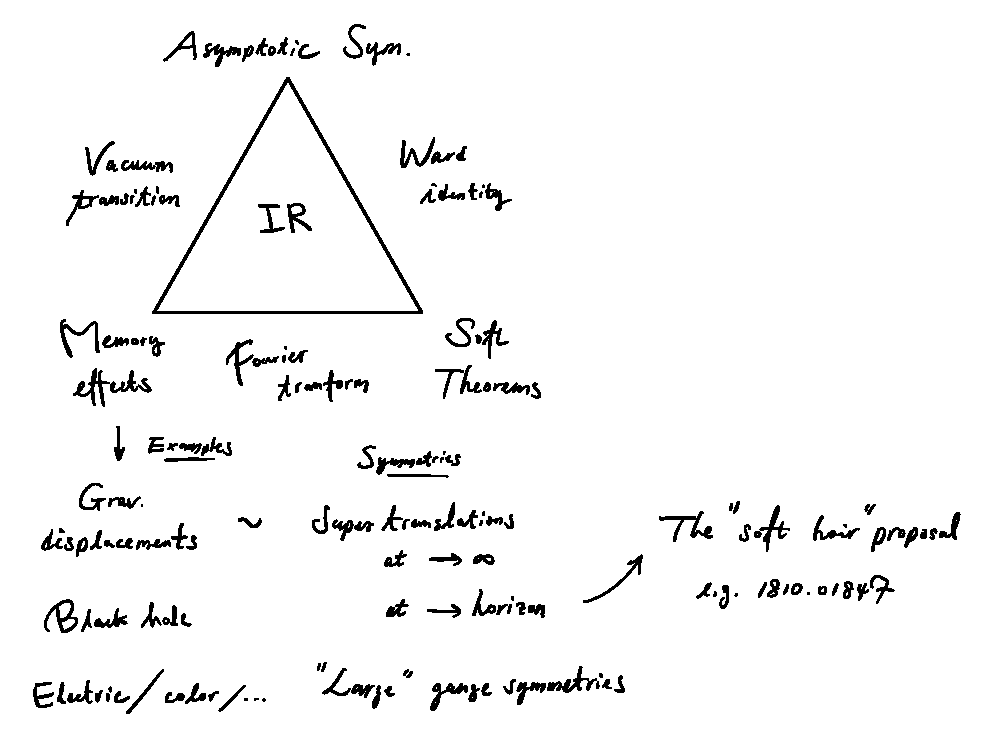
\includegraphics[width=.85\linewidth]{img/IRtriangle.pdf}
	\caption[The universal IR triangle]{
		The universal IR triangle, modeled after the one in \cite{Strominger:2017zoo}. 
	}
	\end{figure}
	
	\end{enumerate}
	
\section{Massless Scattering}
	
	IR divergences in QED: Every time we breathe, an infinite number of soft photons and gravitons are produced. Usual resolution in QFT: cutoff \& resummation of diagrams, but it's hard to understand why it works; the reason: symmetries!
	\begin{figure}[!ht]
	\centering
	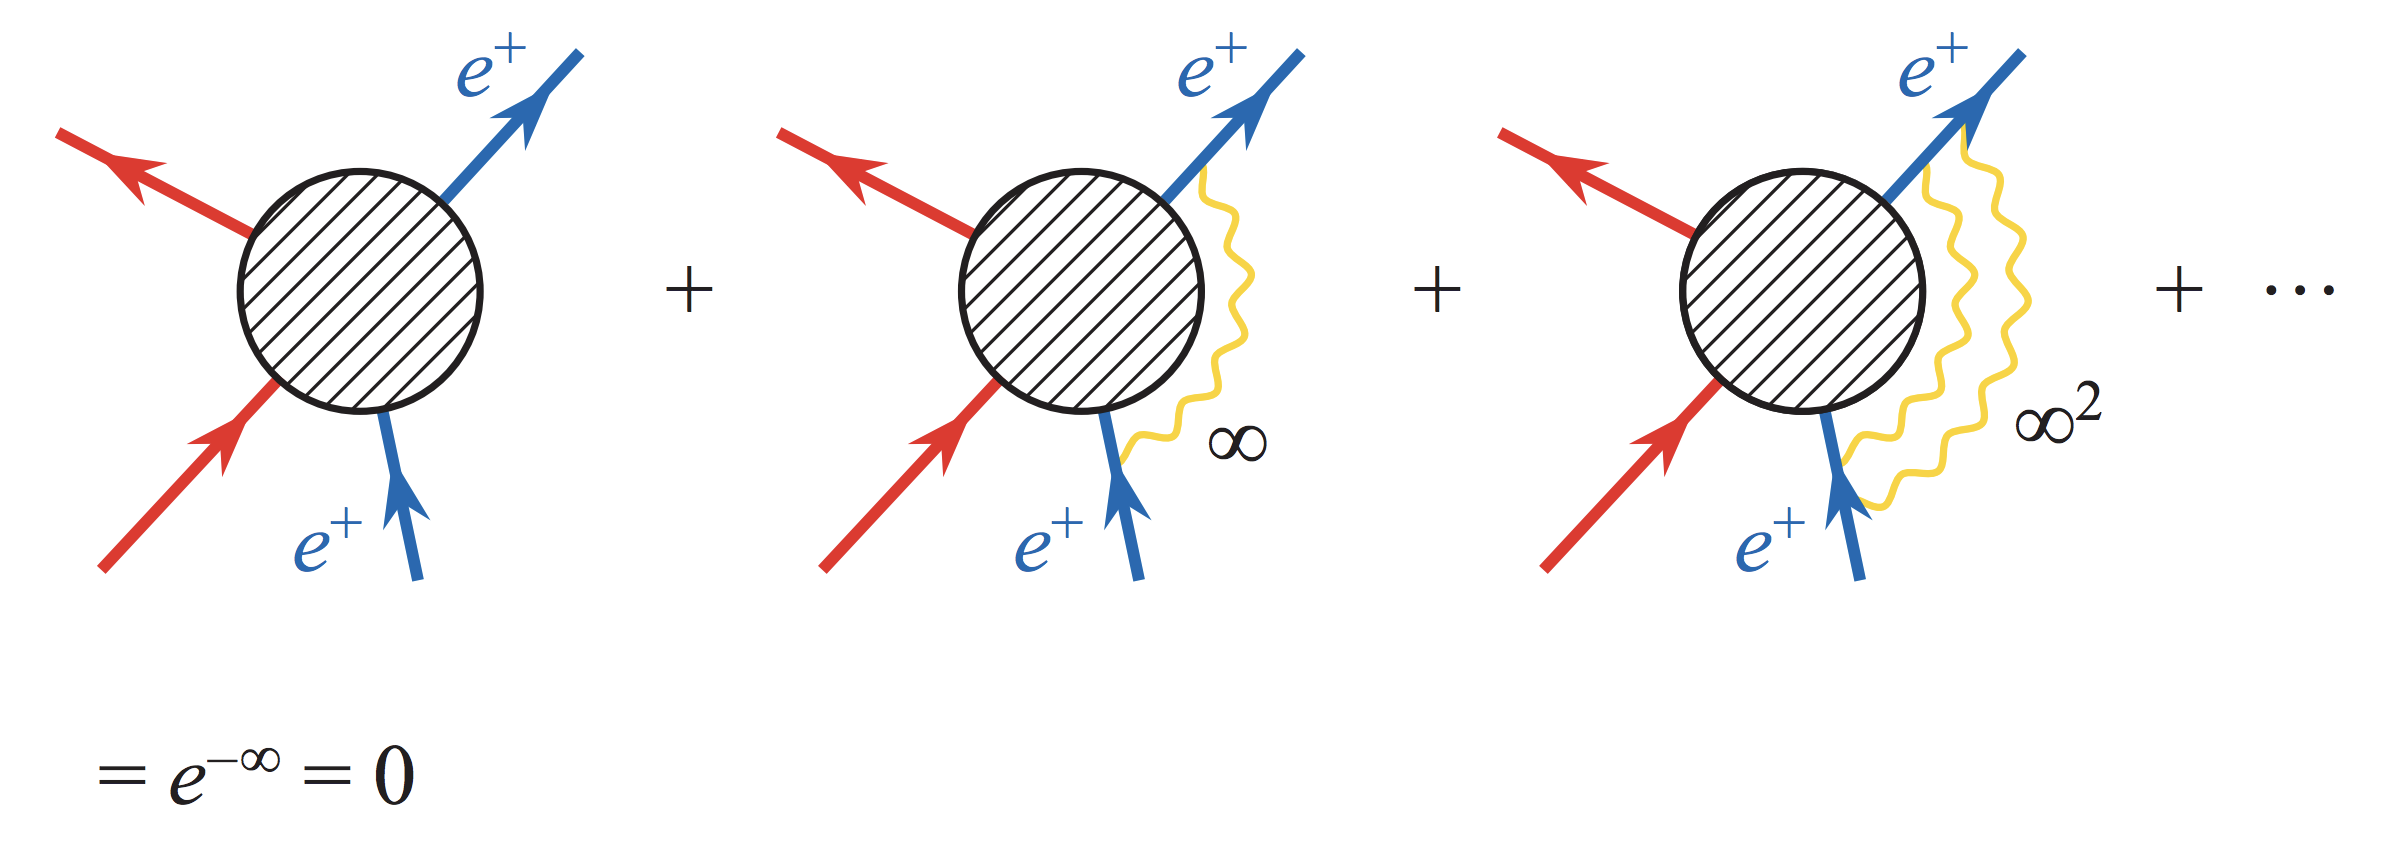
\includegraphics[width=.7\linewidth]{img/Resum.png}
	\caption[Resummation cures IR divergences]{
		Resummation cures IR divergences in the usual diagrammatic analysis of QFT; this is an illustration of the amplitude for Bhabha scattering, taken from \cite{Strominger:2017zoo}. 
		
		Such infinite sum of infinites doesn't make sense mathematically, but this procedure can be made more rigorous with the help with \textit{renormalization}, as we add counterterms to suppress each divergence. 
	}
	\end{figure}
	
	Antipodal identification $\to \infty$ amount of conserved charge (in the IR limit). Consider any function $\epsilon$ on Minkowski space such that:
	\begin{equation}
		\epsilon
		= \epsilon(u,z,\bar{z})|_{\mscr{I}^+}
		= \epsilon(v,z,\bar{z})|_{\mscr{I}^-}
	\end{equation}
	In particular, it obeys the boundary condition near $i^0$:
	\begin{equation}
		\epsilon(u,z,\bar{z})|_{\mscr{I}^+\to i^0}
		= \epsilon(z,\bar{z})
		= \epsilon(v,z,\bar{z})|_{\mscr{I}^-\to i^0}
	\end{equation}
	
	With such $\epsilon(z,\bar{z})$, charge conservation is almost tautological, as both $\epsilon$ and the field $F$ obey the antipodal identification; for example, in QED we have:
	\begin{equation}
	\begin{alignedat}{2}
		Q_\epsilon^-
		:=& \mathrlap{
			\int_{\mscr{I}^-} \Big\{
				\epsilon(v,z,\bar{z})\,
					(\hodgedual j)
				+ \dd{\epsilon}
					\wedge \hodgedual F(v,z,\bar{z})
			\Big\}
		} \\
		=& \int_{\mscr{I}^-}
			\dd{\Bqty\Big{
				\epsilon\,
				(\hodgedual F)
			}}
		&{}=& \int_{CS_{\mscr{I}^-\to i^0}}
			(\hodgedual F)(v,z,\bar{z})\,
			\epsilon(v,z,\bar{z})\big|_{
				v\to +\infty
			} \\
		&&=& \int_{CS_{\mscr{I}^-\to i^0}}
			(\hodgedual F)(z,\bar{z})\,
			\epsilon(z,\bar{z}) \\
		&&=& \int_{CS_{\mscr{I}^+\to i^0}}
			(\hodgedual F)(u,z,\bar{z})\,
			\epsilon(u,z,\bar{z})\big|_{
				u\to -\infty
			}
		= Q_\epsilon^+
	\end{alignedat}
	\end{equation}
	Here we've used Gauss law (Stokes' theorem), and we've assumed no flux due to massive particles passes through the $i^\pm$ endpoints. With $\epsilon = \mrm{const.}$ we recover charge conservation; with general $\epsilon(z,\bar{z})$ we can construct $\infty$ many conserved charges.
	
	In the above derivation we've taken a general $\epsilon(u,z,\bar{z})$ and $\epsilon(v,z,\bar{z})$ defined near $\mscr{I}^\pm$, but note that as the charge reduced to a codim-2 integral on the $CS$ closed to $i^0$, only the angular dependence $\epsilon = \epsilon(z,\bar{z})$ survived; this function actually corresponds to the \textbf{asymptotic symmetries} of QED. 
	
	Our derivation here is similar to some popular treatment of conformal symmetries (see e.g.\ \textit{Polchinski} \cite{Polchinski:1998rq}, section 2.4): we first formally construct a conserved current, in this case:
	\begin{equation}
		\hodgedual J
		= \epsilon(v,z,\bar{z})\,
				(\hodgedual j)
			+ \dd{\epsilon}
				\wedge \hodgedual F(v,z,\bar{z})
		= \dd{(\hodgedual k)},
	\quad
		(\hodgedual k) = \epsilon\,(\hodgedual F)
	\end{equation}
	This conserved current actually gets reduced to the conserved 2-form $\hodgedual k$, and the charge is integrated at a codim-2 surface. This is a common feature of gauge fields. And then, we try to find the corresponding asymptotic symmetries; this is like running the Noether's procedure backwards. After promoting $Q_\epsilon$ to an operator, we see that the asymptotic gauge symmetries are indeed generated by $\epsilon(z,\bar{z})$, and the $u,v$-dependence drops out:
	\begin{equation}
		r\to\infty,
	\quad
		i\var_\epsilon A_\mu
		\equiv \bqty{
			Q_\epsilon, A_\mu
		}
		= i \pdd{\mu} \epsilon,
	\quad \epsilon = \epsilon(z,\bar{z})
	\end{equation}
	
	
	\begin{figure}[!h]
	\centering
	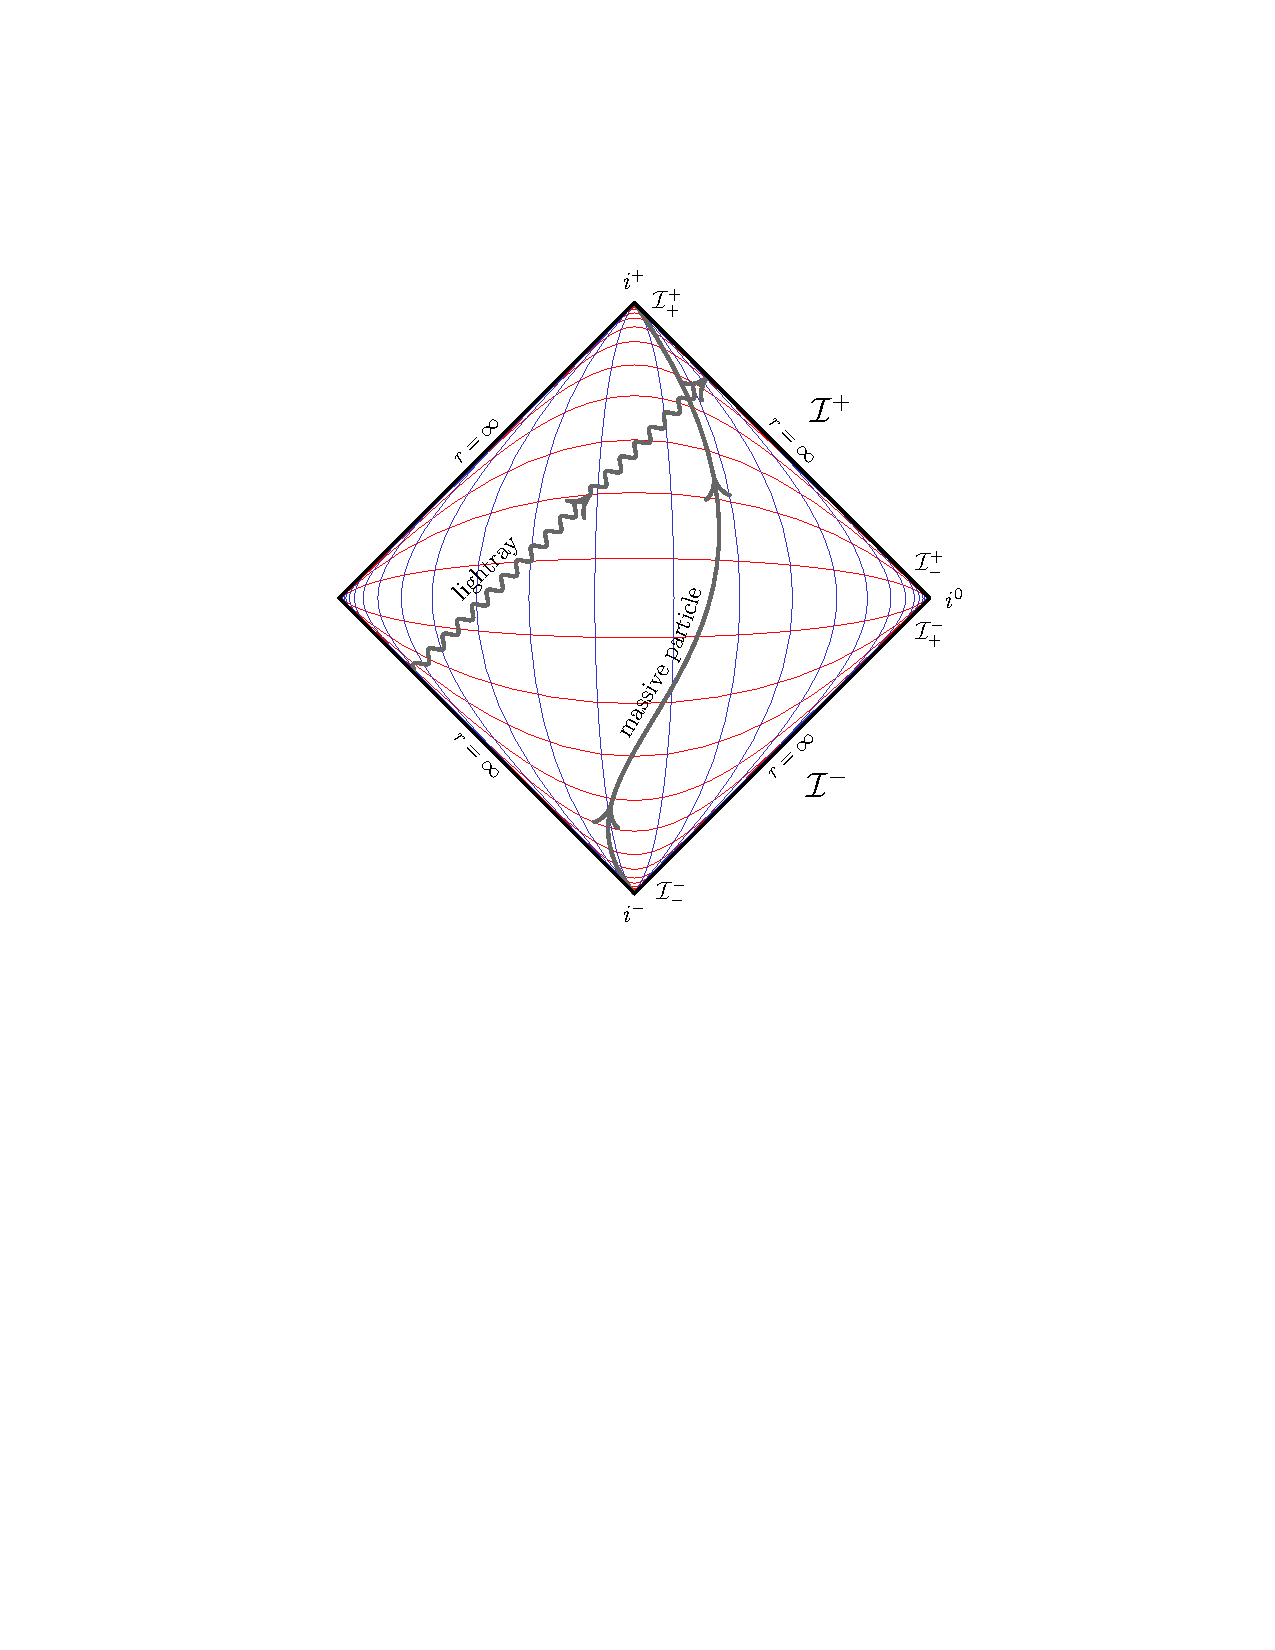
\includegraphics[width=.5\linewidth]{img/minkowskipenrose.pdf}
	\caption[Worldlines of massive and massless particles]{
		Worldlines of massive and massless particles traveling through the Penrose diamond, taken from \cite{Strominger:2017zoo}. Note that the worldlines of massive always pass through $i^\pm$. 
	}
	\end{figure}
	
	Incoming / outgoing asymptotic states are then organized by asymptotic symmetries. If we restrict to massless scattering, $\mscr{I}^\pm$ are nice ``Cauchy surfaces''. 
	The asymptotic states can then be reduced to operator insertions on a celestial sphere $CS$. 
	
	After understanding massless scattering, we can then extend the results carefully to include massive particles, which travels from $i^-$ to $i^+$. The $\mrm{EAdS}$ slicing mentioned above is a nice way to ``regularize'' the singular behavior around $i^\pm$. They correspond to operators that are \textit{smeared} on $CS$. 
	
%\pagebreak[4]
\subsection{Soft theorem \& memory effect}
	Ward identity:
	\begin{equation}
		0
		= \mel{\textsl{out}}{
				\bqty\big{Q_\epsilon, \mcal{S}}
			}{\textsl{in}}
	\end{equation}
	When expanded, gives constraints to the $\mcal{S}$ matrix elements; this gives precisely the \textit{soft theorem}. In fact the $
%		\displaystyle
		\int_{\mscr{I}^+} \Bqty\big{
			\dd{\epsilon}
			\wedge \hodgedual F(u,z,\bar{z})
		}
	$ term creates \textbf{zero energy ``soft'' photons} with transverse polarization $\pdd{\alpha} \epsilon$, $\alpha = z,\bar{z}$, namely it shifts the \textbf{$\infty$-ly degenerate vacuum}. 
	
	The same mechanism leads to the \textbf{memory effect}; one can think of them as same equations for scattering but one in momentum space and the other one in position space. 
	
	\begin{figure}[!h]
	\centering
	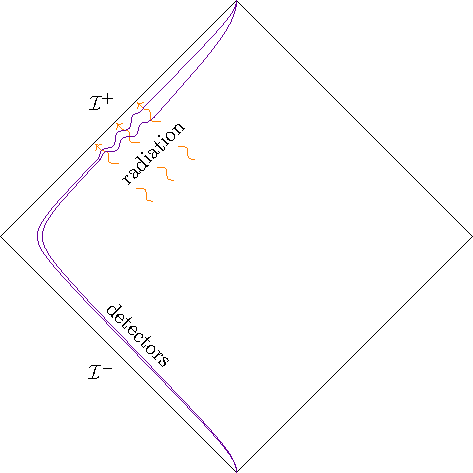
\includegraphics[width=.45\linewidth]{img/memdet.pdf}
	\caption[Gravitational memory effect]{
		Gravitational memory effect, taken from \cite{Strominger:2017zoo}. Amazingly memory effects are very realistic physics and there has been many proposals to measure this in real experiments, both for gravitational memory and other memory effects.
	}
	\end{figure}
\subsection{More on asymptotic symmetries}
	
	Boundary conditions: suitable choice of asymptotic falloffs and gauge conditions; 
	\begin{equation}
		\mrm{ASG}
		= \frac{
			\textsl{allowed gauge symmetries: repect boundary conditions}
		}{
			\textsl{trivial gauge symmetries: act trivially on boundary data (charges)}
		}
	\end{equation}
	e.g.~In asymptotically flat 4D gravity, if we restrict to Lorentz plus ``small translations'', we obtain $\mrm{BMS}_4 = \mrm{BMS}^+ \times \mrm{BMS}^- \supset \text{Poincar\'e}$, i.e.~it is \textbf{$\infty$-ly larger} than the isometry of Minkowski!
	
	However, this is not the full story yet; the conventional BMS is ``both too big and too small'' \cite{Strominger:2017zoo}: ``too big'' because $\mrm{BMS}^+$ and $\mrm{BMS}^-$ should in fact be bound together by the antipodal map; what remains is only the diagonal subgroup; ``too small'' because we can generalize Lorentz transformations to \textit{superrotations}, just like we generalize translations in Poincar\'e to \textit{supertranslations} in BMS. 
	
	Note that according to \cite{Strominger:2017zoo}, analyses of ASG are ``more of an art than a science'', in part because of ambiguities in the choice of boundary conditions, which are often only a posteriori justified. 
	
	Let's first see in detail how we find $\mrm{BMS}^+$. We fix Bondi gauge, which is just \eqref{eq:metric_null_plus} plus small fluctuations with desired falloffs, and then solve the Killing equation:
	\begin{equation}
		\ldv{\zeta} g = 0
	\end{equation}
	Naturally $\zeta \in \mfrak{so}(3,1)$ is part of the solutions, i.e~the 6 Lorentz generators; these are large $\order{r}$ Killing vectors around $\mscr{I}^\pm$. 
	We then consider \textbf{small transformations} around $\mscr{I}^+$, by imposing that the vector field is $\order{1}$ at large $r$ in an orthonormal frame. 
	\begin{equation}
		\zeta^u,\zeta^r
		\sim \order{1},
	\quad
		\zeta^z,\zeta^{\bar{z}}
		\sim \order{\frac{1}{r}}
	\end{equation}
	
	The solution of the Killing equation is then given by an $\infty$-ly generated \textbf{supertranslations} parametrized by $\epsilon = \epsilon(z,\bar{z})$,
	\begin{equation}
		\zeta
		= \epsilon\,\pdd{u}
		- \frac{1}{r} \pqty{
			(\nabla^z \epsilon)\,\pdd{z}
			+ (\nabla^{\bar{z}} \epsilon)\,\pdd{\bar{z}}
		} + (\nabla^2 \epsilon)\,\pdd{r},
	\quad
		\epsilon = \epsilon(z,\bar{z})
	\end{equation}
	We have $\mrm{BMS}^+ = \mrm{Supertranslations}^+ * \mrm{Lorentz}$. Similar result holds for $\mrm{BMS}^-$. If we relax the ``small'' restrictions for $\zeta$, we find that the Lorentz part gets enhanced to \textbf{superrotations}:
	\begin{equation}
		\zeta
		= Y^z \pdd{z}
			+ \frac{u}{2}\,(\nabla_z Y^z)\,\pdd{u}
			+ (\textsl{complex conjugates}),
	\quad
		Y^z = Y^z(z),\ %
		Y^{\bar{z}} = Y^{\bar{z}}(\bar{z})
	\end{equation}
	
	The calculation of conserved charges in gravity is similar to that in gauge theory, but now we already have the symmetry in terms of diffeomorphic generators, thus we need only run the usual Noether's procedure (``forwards'' instead of ``backwards'', compared with what we did in gauge theory), to get the conserved charges. 
	
	Again we integrate the conserved current on the codim-1 $\mcal{I}^\pm$, and it gets reduced to an integral of the codim-2 $CS$ near $i^0$. $\epsilon = 0$ corresponds to $\zeta \propto \pdd{u}$, and the conserved charge is the \textbf{total Bondi mass}; for Kerr spacetimes in the usual conventions, the conserved charge is exactly the mass parameter $M$. 
	
	\begin{figure}[!t]
	\centering
	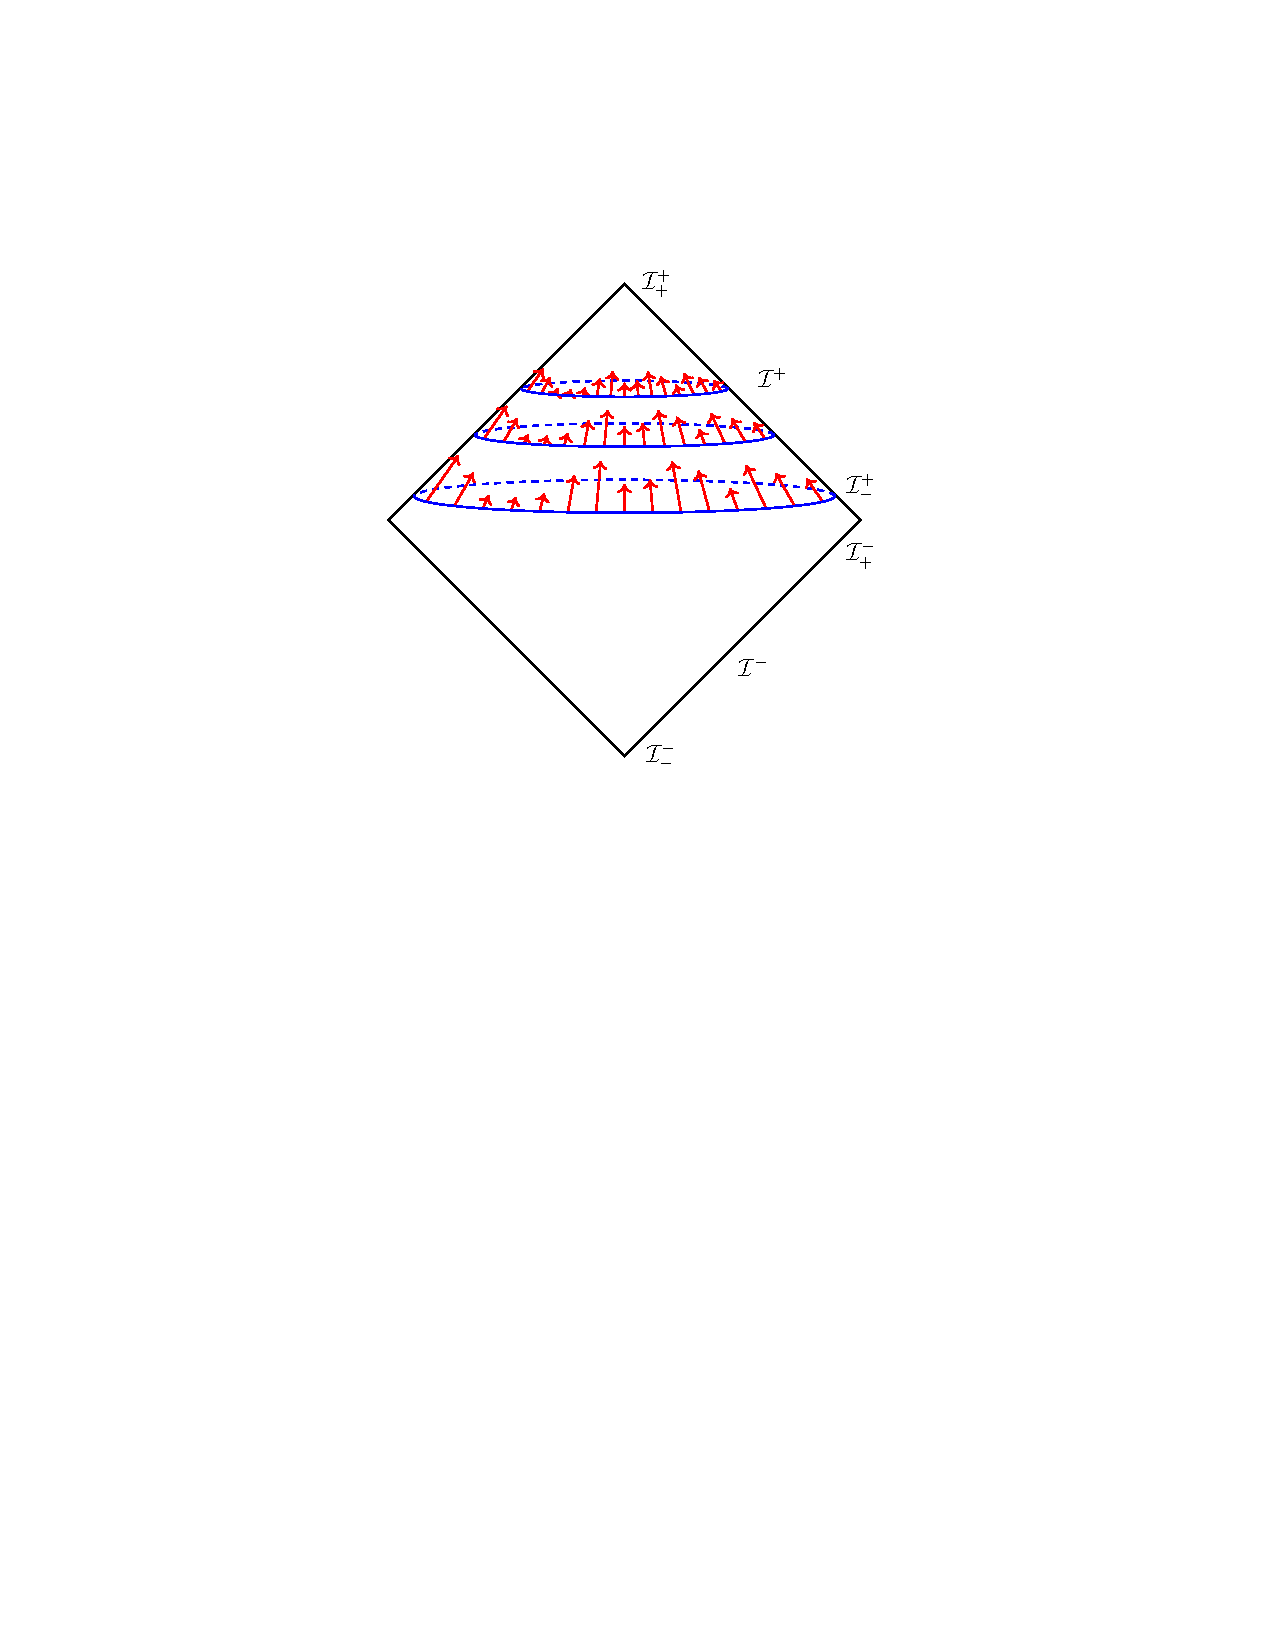
\includegraphics[width=.45\linewidth]{img/supertranslation.pdf}
	\caption[Supertranslations on $\mscr{I}^+$]{
		Supertranslations on $\mscr{I}^+$, taken from \cite{Strominger:2017zoo}.
	}
	\end{figure}
	
%\pagebreak[4]
\subsection{Scattering on the celestial sphere}
	
	\begin{figure}[!ht]
	\centering
	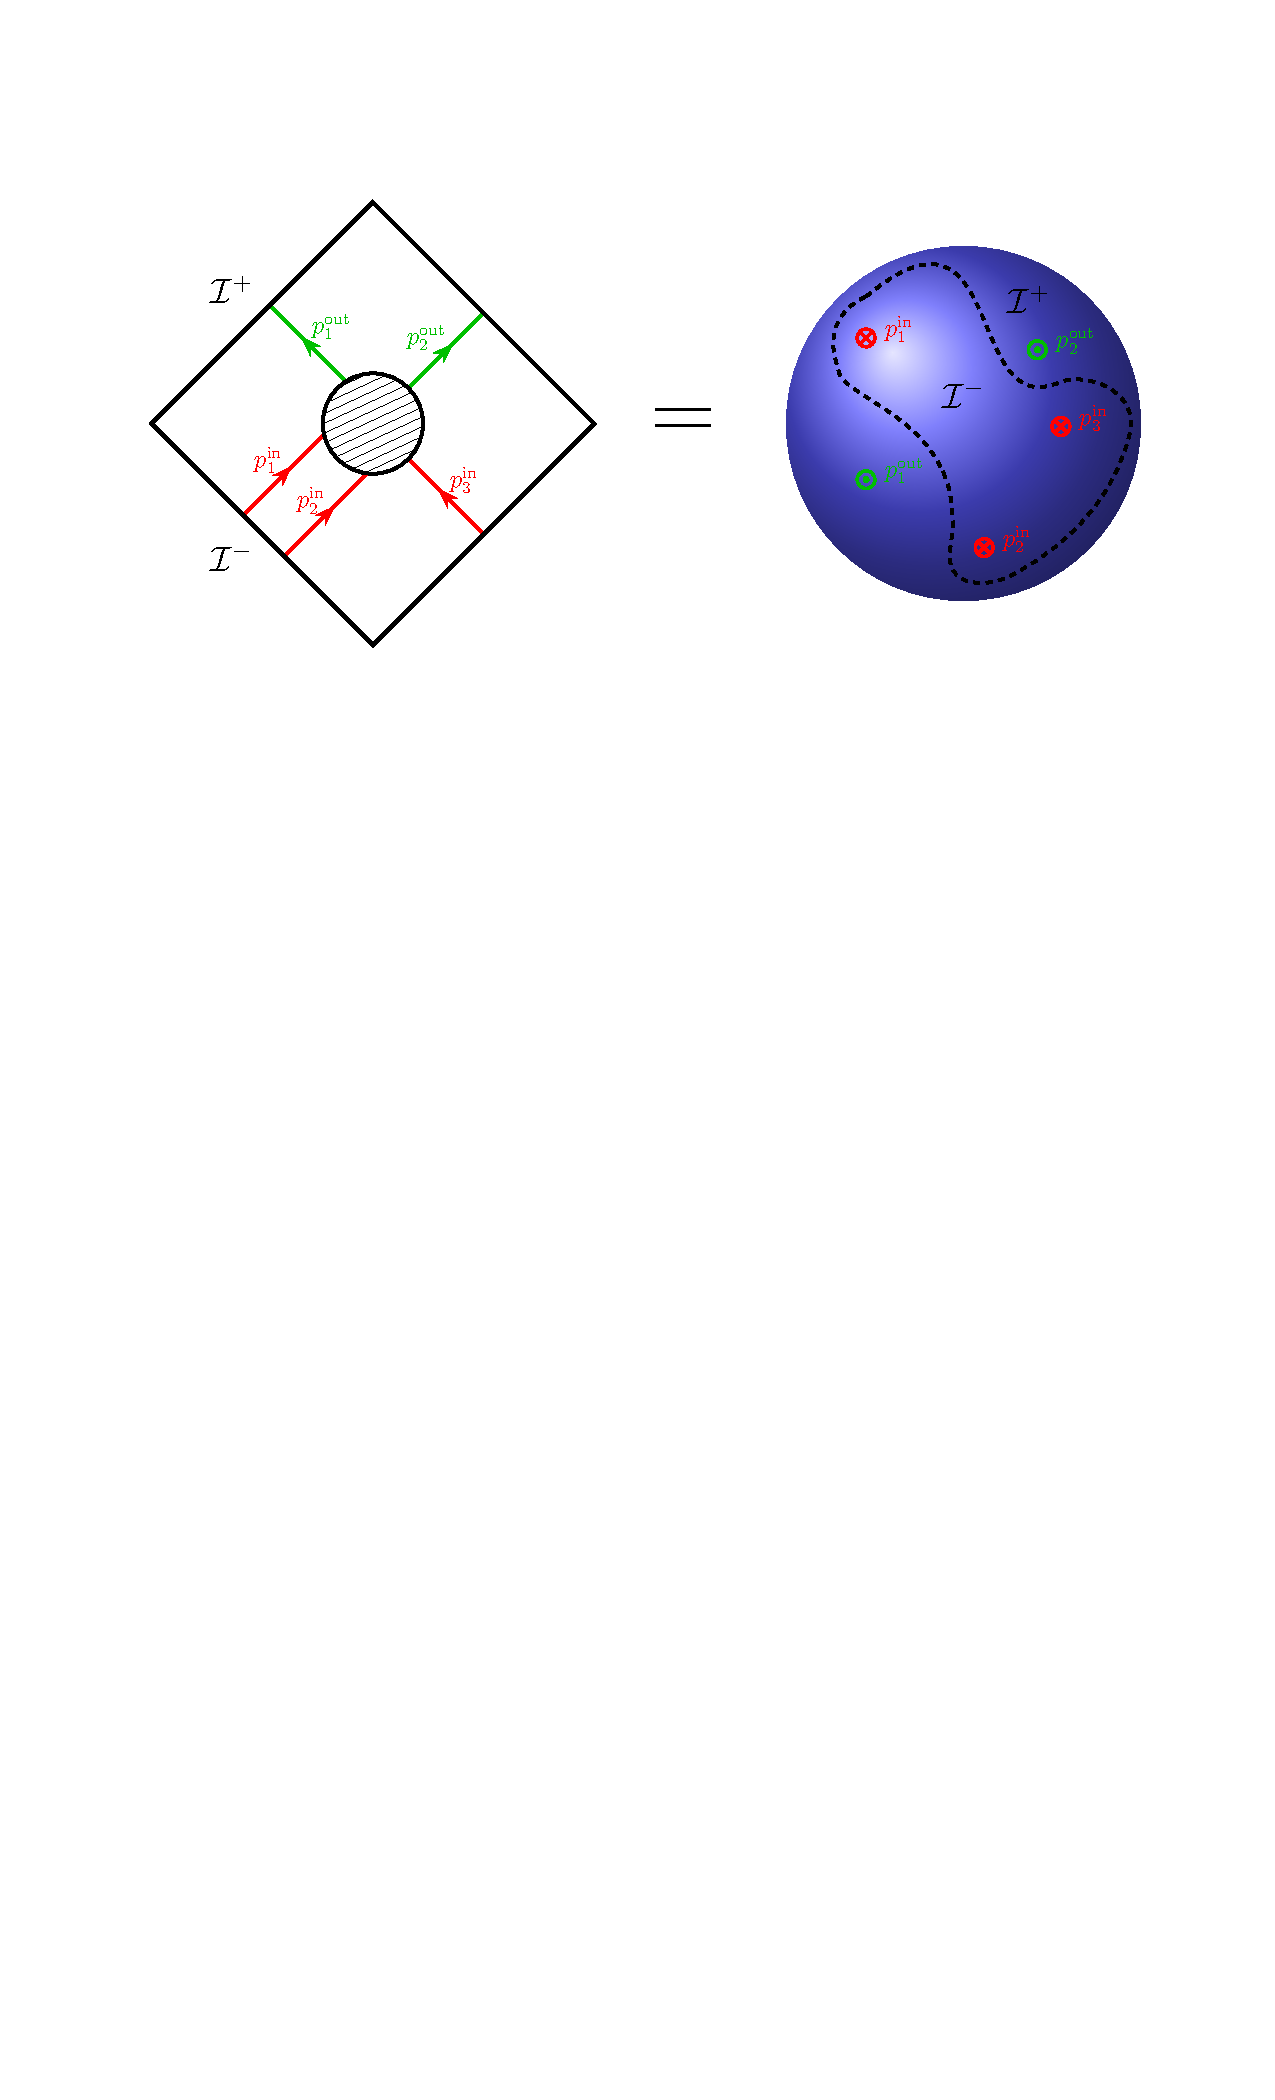
\includegraphics[width=.7\linewidth]{img/celestialsphere.pdf}
	\caption[Scattering on the celestial sphere]{
		Scattering reduced onto the celestial sphere, taken from \cite{Strominger:2017zoo}.
	}
	\end{figure}
	
\pagebreak[3]
	
	Usually we use 4-\textbf{energy momentum} $P_\mu$ to label asymptotic states, but for massless particles it's more natural to use \textbf{boosts} \cite{Pasterski:2017kqt,Pate:2019mfs}: note that a boost along $\vec{p}$ of a null $p^\mu = (\abs{\vec{p}},\vec{p})$ only rescales its magnitude: $p^\mu\mapsto \lambda p^\mu$. This corresponds to \textbf{dilations} on the celestial CFT. 
	\begin{equation}
		T\sim \pdd{x},
	\quad
		\tilde{f}(p)
		\sim \int \dd{x} e^{-ipx} f(x)
	\end{equation}
	\vspace{-.5\baselineskip}
	\begin{equation}
		B\sim \omega\,\pdd{\omega},
	\quad
		\tilde{f}(\Delta)
		\sim \int \frac{\dd{\omega}}{\omega}\,
				\omega^\Delta f(\omega),
	\quad
		p^\mu = \epsilon\,\omega\, q^\mu(z,\bar{z})
	\end{equation}
	$q^\mu = \pqty{
		1 + z\bar{z},
		z + \bar{z},
		-i(z - \bar{z}),
		1 - z\bar{z}
	}$ is a standard 4-momentum constructed only with the celestial direction $(z,\bar{z})$. $\omega$ is the energy (frequency), and $\epsilon = \pm 1$ (for outgoing and ingoing particles respectively. 
	This is a so-called \textbf{Mellin transform}, with boost weight: $\Delta$. 
	
	When combined with spin, we can similarly define $(h,\bar{h})$ for the 2D celestial sphere, $\Delta = h + \bar{h}$; \textit{Conformally soft}: $h\to 0$ or $\bar{h}\to 0$. Soft theorem $\to$ conformal soft theorem; see \cite{Pate:2019mfs}. 
	
\appendix
\section{Symmetries of asymptotically flat spacetime}
	\vspace{-.5\baselineskip}
	\begin{center}
	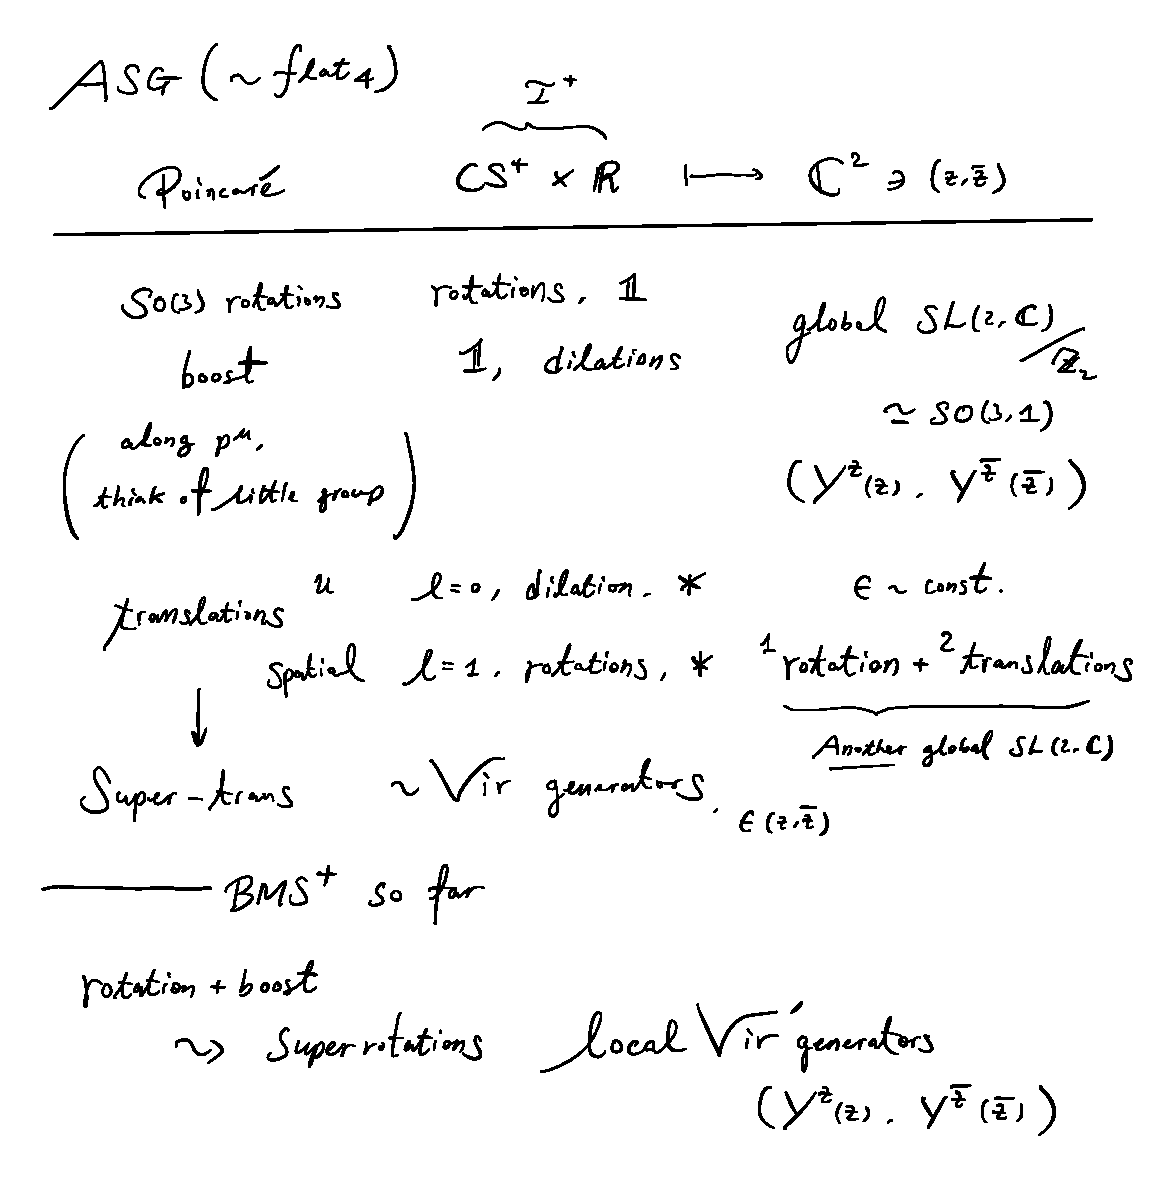
\includegraphics[width=.85\linewidth]{img/ASGflat.pdf}
	\end{center}
	

\vspace{1.2\baselineskip}
\raggedright
\printbibliography[%
%	title = {参考文献} %
	,heading = bibintoc
]
\end{document}
